\documentclass[nonacm=true, language=german]{acmart}

\usepackage{booktabs}
\usepackage{multirow}
\usepackage{makecell}

\usepackage{dirtytalk}
\usepackage{nameref}

\usepackage{tikz}
\usetikzlibrary{graphs}
\usetikzlibrary{shapes.geometric}

\tikzstyle{node} = [minimum height=1.5cm, text centered, align=center]
\tikzstyle{input} = [node, diamond, minimum width=3.5cm, fill=red!30]
\tikzstyle{feature} = [node, ellipse, minimum width=2cm, fill=blue!30]
\tikzstyle{method} = [node, minimum width=2.5cm, fill=orange!30, rounded corners]

\newcommand{\tabitem}{~~\llap{\textbullet}~~}
\newcommand{\set}[1]{\{#1\}}
\newcommand{\attack}[3]{#1 \, #2 \, #3}
\renewcommand{\not}[1]{not \, #1}

%\setcounter{tocdepth}{3}

\title{Intelligente Systeme}

\subtitle{Zusammenfassung}

\author{Per Natzschka}

\email{per.natzschka1@mailbox.tu-dresden.de}

\begin{document}

\maketitle

\tableofcontents

\newpage
\section{Suche}

\subsection{Klassifizierung}

\subsubsection{Parameter}

\begin{itemize}
    \item $b$: max. Verzweigungsfaktor (branching factor)
    \item $d$: Tiefe der besten Lösung (depth)
    \item $m$: max. Tiefe des Baumes (kann $ \infty $ sein)
\end{itemize}

\subsubsection{Bewertung}

\begin{itemize}
    \item Zeitkomplexität: Zahl expandierter Knoten?
    \item Speicherkomplexität: Zahl an Knoten im Speicher?
    \item Vollständigkeit: findet Lösung?
    \item Optimalität: findet beste Lösung?
\end{itemize}

\subsection{Uninformierte Suche}

\subsubsection{Breiten- und Tiefensuche}

\text{}

\begin{table}[ht]
    \centering
    \begin{tabular}{c|c c c c}
        \toprule
        Strategie           & \makecell{Breitensuche \\ BFS}    & \makecell{Tiefensuche \\ DFS}                                 & \makecell{Tiefenbeschränkte \\ Suche} & \makecell{Iteratives \\ Vertiefen} \\
        \midrule
        Datenstruktur       & FIFO                              & FILO                                                          & FILO                                  & FILO \\
        Zeitkomplexität     & $ O(b^d) $                        & $ O(b^m) $                                                    & $ O(b^t) $                            & $ O(b^d) $\\
        Speicherkomplexität & $ O(b^d) $                        & $ O(b \cdot m) $                                              & $ O(b \cdot t) $                      & $ O(b \cdot d) $ \\
        Vollständigkeit     & ja, wenn $b$ endlich              & \makecell{ja, wenn $d$ endlich \\ und Schleifenüberprüfung}   & ja, wenn $ d \leq t $                 & \makecell{ja, wenn $ d < \infty $ \\ und $ b < \infty $} \\
        Optimalität         & \checkmark (wenn $b$ endlich)     & $\times$                                                      & $\times$                              & \checkmark \\
        \bottomrule
    \end{tabular}
    \caption{Vergleich Breiten- und Tiefensuche}
    \label{tab:bfs_dfs}
\end{table}

\subsubsection{Uniforme Kostensuche}

\begin{itemize}
    \item Dijkstra
    \item expandiere immer Knoten mit geringsten Kosten von der Wurzel
    \item optimal
    \item vollständig
\end{itemize}

\subsection{Informierte Suche}

\begin{table}[ht]
    \centering
    \begin{tabular}{c|c c}
        \toprule
        Strategie           & Greedy-Suche                                      & A*-Suche \\
        \midrule
        Vollständigkeit     & \multicolumn{2}{c}{ja, bei Schleifenüberprüfung} \\
        Zeitkomplexität     & $ O(b^m) $                                        & $ O(b^m) $ \\
        Speicherkomplexität & $ O(b^m) $                                        & $ O(b^m) $ \\
        Optimalität         & $ \times $                                        & \checkmark (wenn $h$ zulässig) \\
        \bottomrule
    \end{tabular}
    \caption{Vergleich informierter Suchstrategien}
    \label{tab:informed_search}
\end{table}

\begin{itemize}
    \item Heuristik
    \begin{itemize}
        \item $ h: V \to \mathbb{R} $
        \item schätzt Kosten von Knoten zum Ziel
        \item $ h(Ziel) = 0 $
        \item $ \forall_{n \in V}: h(n) \geq 0 $    
    \end{itemize}
    
    \item Zulässige Heuristik:
    \begin{itemize}
        \item $ \forall_{n \in V}: h(n) \leq h^*(n) $
        \item $h^*$ sind wahre Kosten
    \end{itemize}
    
    \item Konsistente Heuristik
    \begin{itemize}
        \item $ \forall_{n, n' \in V}: h(n) \leq c(n, n') + h(n') $
        \item $n'$ ist Nachfolger von $n$
        \item $ c(n, n') $ sind Kosten für Übergang $ n \to n' $
        \item immer zulässig
    \end{itemize}
\end{itemize}

\subsubsection{Greedy Suche}

Knoten mit geringster Distanz zum Ziel wird zuerst expandiert.

$$ v_{next} = arg\,min_{v \in V}h(v) $$

\subsubsection{A*-Suche}

\begin{itemize}
    \item neben $h$ auch bisherige Kosten $ g: V \to \mathbb{R} $ einberechnet
    \item Kostenfunktion $ f: V \to \mathbb{R}, n \mapsto g(n) + h(n) $.
    \item gegen Speicherüberlauf: Schwellwert $K$
    \begin{itemize}
        \item $K \geq K* $
        \item $K^*$ sind wahre Kosten
        \item Knoten mit $ f(n) > K $ werden nicht besucht
        \item Bestimmung von $K$ durch nichtoptimalen Algorithmus (z. B. Greedy)
    \end{itemize}
\end{itemize}

\newpage
\section{Entitätenerkennung}

\begin{table}[ht]
    \centering
    \begin{tabular}{c|c c}
        \toprule
        Strategie & Vorteile  & Nachteile \\
        \midrule
        Lexikon &
        \makecell{
         \tabitem einfach \\
         \tabitem schnell
        }
        & 
        \makecell{
         \tabitem Mehrdeutigkeiten nicht erkannt \\
         \tabitem Vollständigkeit nicht garantiert \\
         \tabitem Pflege (keine Abstraktionen/Muster)
        }
        \\
        \midrule
        \makecell{Reguläre \\ Ausdrücke}    &
        \makecell{
         \tabitem kompakte Repräsentation
        }
        & 
        \makecell{
         \tabitem Woher kommt Ausdruck? \\
         \tabitem manuelle Definition/Debugging mühsam \\
         \tabitem Mehrdeutigkeiten nicht erkannt
        }
        \\
        \midrule
        \makecell{Rand- \\ klassifikator}   &
        \makecell{
         \tabitem Mehrdeutigkeiten teilweise \\ aufgelöst (lokaler Kontext)
        }
        & 
        \makecell{
         \tabitem Qualität von Trainingsdaten \\
         \tabitem Auswahl von Merkmalen
        }
        \\
        \midrule
        Token-Fenster   &
        \makecell{
         \tabitem Mehrdeutigkeit aufgelöst \\ (lokaler Kontext)
        }
        & 
        \makecell{
         \tabitem Qualität von Trainingsdaten \\
         \tabitem Auswahl von Merkmalen
        }
        \\
        \midrule
        \makecell{Hidden Markov \\ Models (HMM)}    &
        \makecell{
         \tabitem Mehrdeutigkeit aufgelöst
        }
        & 
        \makecell{
         \tabitem Qualität von Trainingsdaten
        }
        \\
        \bottomrule
    \end{tabular}
    \caption{Vergleich der Strategien zur Entitätenerkennung}
    \label{tab:entity_recognition}
\end{table}

\begin{itemize}
    \item Wissensakquise
    \begin{itemize}
        \item per Hand
        \item Regeln lernen (Entscheidungsbäume)
        \item Natürliche Sprachverarbeitung
    \end{itemize}
    
    \item Informationsextraktion
    \begin{enumerate}
        \item Entitäten lokalisieren
        \item Entitäten klassifizieren
        \item Fakten extrahieren
    \end{enumerate}
    
    \item Probleme
    \begin{itemize}
        \item Sprachlich
        \begin{itemize}
            \item lexikalisch (tumor $\leftrightarrow$ tumour)
            \item orthographisch ($\alpha$-helix $\leftrightarrow$ alpha-helix)
            \item strukturell (lung cancer $\leftrightarrow$ cancer of the lung)
            \item morphologisch (kick $\leftrightarrow$ kicked)
        \end{itemize}
        
        \item Mehrdeutigkeit (Siemens, Paris)
        \item Anaphora
        \begin{itemize}
            \item Pronomen
            \item Proformen (Er fliegt nach Paris. Er will \textit{dort} Urlaub machen.)
            \item Bridging (Der Motor ist kaputt. Der Keilriemen ist gerissen $\leftrightarrow$ Der Motor ist kaputt. Der Schnürsenkel ist gerissen.)
        \end{itemize}
        
        \item Metonymie/Vertauschung (Schiller lesen)
        \item Synekdoche (Ober-/Überbegriffe)
    \end{itemize}
    
    \item Text preprocessing
    \begin{itemize}
        \item Format
        \item Satzgrenzen
        \item Tokenisierung
        \item Stemming
    \end{itemize}
\end{itemize}

\begin{itemize}
    \item direkte Suche linear in
    \begin{itemize}
        \item Textgröße
        \item Zahl der Lexikoneinträge
        \item Länge der Lexikoneinträge
    \end{itemize}
    
    \item Boyer-Moore (basically KMP)
    \item Zipf's Law
    \begin{itemize}
        \item Worte nach Häufigkeit sortieren
        \item Wahrscheinlichkeit eines Wortes invers proportional zu Rang
    \end{itemize}
    
    \item Trie
    \begin{itemize}
        \item Baum
        \item $n$-te Verzweigung $\leftrightarrow$ $n$-ter Buchstabe
    \end{itemize}
    
    \item Radix-Tree
    \begin{itemize}
        \item wie Trie
        \item Verzweigungen mit Teilwörtern
    \end{itemize}
    
    \item Levenshtein-Distanz
    \begin{itemize}
        \item Top-Down-Implementierung: $O(2^n)$
        \item Bottom-Up-Implementierung: $O(n^2)$ (dynamisches Programmieren, u. a. Speicherung der Zwischenwerte in Matrix)
    \end{itemize}
    
    \item Dice-Koeffizient
    \begin{itemize}
        \item Betrachtung v. Trigrammen
        \item $ t(Peter) = \set{Pet, ete, ter} $
        \item $ dice(a, b) = 2 \cdot \frac{|t(a) \, \cap \, t(b)|}{|t(a)| \, + \, |t(b)|} \in [0, 1] $
        \item Reihenfolge geht verloren
    \end{itemize}
\end{itemize}

\subsection{Klassifikatoren}

\subsubsection{Randklassifikator}

\begin{itemize}
    \item Klassifiziere Leerstellen zwischen Token
    \begin{itemize}
        \item Anfang und Ende von Entitäten
        \item Satzgrenzen
    \end{itemize}
    
    \item Leerstellen als Vektoren von Merkmalen, z. B.:
    \begin{itemize}
        \item nächstes Token beginnt mit Großbuchstaben
        \item vorheriges ist Zahl
        \item vorheriges ist \say{in}
    \end{itemize}
\end{itemize}

\subsubsection{Token-Fenster}

\begin{itemize}
    \item Klassifikation anhand von Kontextfenster
    \item Fenstergröße?
    \item Merkmale?
    \begin{itemize}
        \item Token, Stämme, POS-Tags
        \item n-grams
        \item Präfixe/Suffixe
        \item Vorher vergebene Klassen
    \end{itemize}
    
    \item Lernen anhand von Merkmalsvektoren aus Beispielen
\end{itemize}

\subsubsection{Hidden Markov Models}

\begin{itemize}
    \item Markov-Modelle
    \begin{itemize}
        \item probabilistische Modelle
        \item modellieren Zustandsübergänge
        \item nur von aktuellem Zustand abhängig
    \end{itemize}
    \item Hidden Markov Models
    \begin{itemize}
        \item Zustände selbst nicht betrachtet
        \item Übergangswahrscheinlichkeiten abhängig von allen vorherigen Zuständen
    \end{itemize}
    
    \item $ \Theta = (S, \Sigma, A, B, \Pi)$
    \begin{itemize}
        \item $S$: Zustände (semantische Klassen/Labels)
        \item $\Sigma$: Alphabet (Beobachtungen/Tokens)
        \item $A$: Übergangswahrscheinlichkeiten
        \item $B$: Emissionswahrscheinlichkeiten
        \item $\Pi$: Anfangszustandswahrscheinlichkeiten
    \end{itemize}
    
    \item Wahrscheinlichkeiten an Trainingsdaten gelernt
    \item Wahrscheinlichkeit von Beobachtungssequenz $o$ und Zustandssequenz $s$: $P(s \cap o)$
    \begin{itemize}
        \item $ P(s \cap o) = P(o | s) P(s) $
        \item $ P(s \cap o) \propto P(o_0 | s_0) P(s_0) \displaystyle \prod_{t=1}^{|o|} P(o_t | s_t) P(s_t | s_{t-1}) $
    \end{itemize}
    
    \item Bestimmung der besten Lösung durch $ arg \, max_s P(s, o) \rightarrow $ ineffizient
    \item Viterbi-Algorithmus (effizient)
    \begin{itemize}
        \item dynamische Programmierung
        \item Tabelle: $ S \times o $
        \item $ F(i, 0) = \Pi(i) \cdot B(i, 0) $
        \item $ F(i, j) = max_r(F(r, j-1) \cdot A(r, i)) \cdot B(i, j) $
        \item Spaltenweise Berechnung von links nach rechts
    \end{itemize}
\end{itemize}

\subsection{Bewertung}

\begin{itemize}
    \item Precision: $ p = \frac{TP}{TP \, + \, FP} $
    \item Recall: $ r = \frac{TP}{TP \, + \, FN} $
    \item F-Measure: $ 2 \cdot \frac{p \cdot r}{p \, + \, r} $ (Harmonisches Mittel)
    \item $k$-fache Kreuzvalidierung
    \begin{itemize}
        \item Daten in $k$ Gruppen aufgeteilt
        \item Training auf $k-1$ Gruppen
        \item Validierung mit $k.$ Gruppe
    \end{itemize}
\end{itemize}

\newpage
\section{Relationsextraktion}

\begin{table}[ht]
    \centering
    \begin{tabular}{c|c c}
        \toprule
         Strategie  & Vorteile  & Nachteile \\
         \midrule
         \makecell{Maschinelles \\ Lernen}    &
         \makecell{
             \tabitem einfach
         }
         & 
         \makecell{
             \tabitem Qualität von Trainingsdaten \\
             \tabitem Auswahl von Merkmalen
         }
         \\
         \midrule
         Kookkurrenz    &
         \makecell{
             \tabitem einfach \\
             \tabitem hoher Recall
         }
         & 
         \makecell{
             \tabitem kein Relationstyp
         }
         \\
         \midrule
         \makecell{Reguläre \\ Ausdrücke}   &
         \makecell{
             \tabitem hohe Precision \\
             \tabitem Transparenz
         }
         & 
         \makecell{
             \tabitem Generierung
         }
         \\
         \bottomrule
    \end{tabular}
    \caption{Vergleich der Strategien zur Relationsextraktion}
    \label{tab:relation_extraction}
\end{table}

\subsection{Kookkurrenz}

\begin{itemize}
    \item Wie oft treten Begriffe gemeinsam auf?
    \item Signifikanz
    \begin{itemize}
        \item steigt mit gemeinsamen Auftreten
        \item sinkt mit nicht gemeinsamen Auftreten
    \end{itemize}
    
    \item log odds ratio
    \begin{itemize}
        \item $ c(a, b) = \log_2(\frac{n \cdot n_{ab}}{n_a \cdot n_b}) $
        \item $n$ ist Anzahl aller Dokumente
        \item $n_{ab}$ ist Anzahl der Dokumente mit $a$ und $b$
        \item $n_a$ ist Anzahl der Dokumente mit $a$
        \item $\log$ optional/Basis frei wählbar (nur scaling)
    \end{itemize}
\end{itemize}

\subsection{Reguläre Ausdrücke}

\subsubsection{Vorgehen}

\begin{table}[ht]
    \centering
    \begin{tabular}{c c}
        \toprule
        Syntax  & Semantik \\
        \midrule
        $.$             & beliebiges $a \in \Sigma $ \\
        $a*$            & $\set{a}^*$ \\
        $a+$            & $\set{a}^+$ \\
        $a?$            & $\set{\varepsilon, a}$ \\
        $a \, | \, b$   & $\set{a, b}$ \\
        \bottomrule
    \end{tabular}
    \caption{Syntax und Semantik von Regulären Ausdrücken}
    \label{tab:my_label}
\end{table}

\begin{itemize}
    \item Lernen anhand positiver Beispiele von Entitäten in Relation
    \item Zeichenketten zwischen Entitäten
    \item Multiples Sequenzalignement der Zeichenketten
    \item Ableiten eines regulären Ausdrucks
\end{itemize}

\subsubsection{Multiple Sequence Alignement (MSA)}

\begin{itemize}
    \item Dynamische Programmierung
    \begin{itemize}
        \item bei $m$ Wörtern, Levenshtein über $m$ Dimensionen
        \item $m$ Wörter der Länge $n$
        \item $n^m$ Zellen mit jeweils $2^m-1$ Nachbarn
        \item $O(2^m-1)$
    \end{itemize}
    
    \item Optimierung: Greedy (Inkrementelles Positionieren)
    \begin{itemize}
        \item zwei Strings alignen
        \item nächste Strings mit bisherigem Alignement alignen
        \item Kosten bei jedem Schritt inkrementieren
        \item Pro: $O(m \cdot n^2)$
        \item Con: nicht optimal, Reihenfolge der Abarbeitung bestimmt stark das Ergebnis
        \item Heuristik: Reihenfolge der Strings
        \item Clustering der Zeichenketten nach paarweiser Distanz
        \item Reihenfolge basierend auf Clustern (lokales Optimum)
        \item lokales Optimum
    \end{itemize}
    
    \item Optimierung: A* (Optimales Positionieren)
    \begin{itemize}
        \item Knoten: Zellen der Matrix
        \item Kanten: Verbindung benachbarter Zellen
        \item Startknoten: $(0, 0, 0)$
        \item Zielknoten: $(n, n, n)$
        \item Kosten $h^*$: Kosten für multiples Alignement der Reste der Zeichenkette
        \item multiple Alignements schlechter als Summe paarweiser Alignements
        \item Heuristik $h$ ist Summe der Kosten aller paarweisen Alignements
        \item $ h(i_1, \dots, i_m) = \displaystyle \sum_{a, b \, \in \, \set{l_1[i_1:], \dots, l_m[i_m:]}} dist(a, b) $
        \item für Heuristik Betrachtung von $ \frac{m \cdot (m-1)}{2} $ Alignements
    \end{itemize}
\end{itemize}

\newpage
\section{Entscheidungsbäume}

\begin{table}[ht]
    \centering
    \begin{tabular}{c|c}
        \toprule
         Vorteile & Nachteile \\
         \midrule
         \makecell{
             \tabitem einfach, da tabellarisches Wissen oft verfügbar \\
             \tabitem schnell durch Greedy-Ansatz (Entropie) \\
             \tabitem robust durch Random Forests
         }
         & 
         \makecell{
             \tabitem stark von Datenerhebung abhängig \\
             \tabitem Wahl der Atribute \\
             \tabitem Wahl der Wertebereiche
         }
         \\
         \bottomrule
    \end{tabular}
    \caption{Vor- und Nachteile von Entscheidungsbäumen}
    \label{tab:decision_trees}
\end{table}

\begin{itemize}
    \item Entscheidungsbaum
    \begin{itemize}
        \item Innere Knoten: Attribute
        \item Kanten: Wert der Attribute
        \item Blätter: Einteilung der Daten
    \end{itemize}
    
    \item Ziel: möglichst kleiner Entscheidungsbaum
    \begin{itemize}
        \item globales Optimum
        \item lokales Optimum (greedy)
    \end{itemize}
    
    \item Zahl möglicher Bäume mit $m$ Blättern: $T(m)$
    \begin{itemize}
        \item $ T(m) = (2m - 3)!! $
        \item $!!$ ist Doppelfakultät
        \begin{itemize}
            \item $ 1!! := 1 $
            \item $ n!! := n \cdot (n - 2)!! $
        \end{itemize}
    \end{itemize}
    
    \item Rekursives Teilen der Beispiele
    \begin{enumerate}
        \item Teilgruppe ist homogen $\rightarrow$ Knoten erhält Label der Teilgruppe
        \item Teilgruppe ist inhomogen $\rightarrow$ wähle nächstes Attribut
        \item Es gibt keine Attribute mehr $\rightarrow$ Knoten erhält Label der Mehrheit der Teilgruppe
        \item Es gibt keine Beispiele mehr $\rightarrow$ Knoten erhält Label der Mehrheit der Teilgruppe des Elternknotens
    \end{enumerate}
    
    \item \label{entropy} Entropie $H$
    \begin{itemize}
        \item Bewertung der Homogenität einer Menge
        \item $ H(C) = \displaystyle \sum_{i \, \in \, C} -p_i \cdot \log_2(p_i) $
        \item $T$: Menge der Beispiele, $p_i$: Anteil der Beispiele, die zu Klasse $i$ gehören, $C$: Klassen
        \item Informationsgewinn durch Attribut $A$: $ IG(A) = H(T) - R(T) $
        \item Restentropie $ R(T) = \displaystyle \sum _{i=1}^v H(T_i) \cdot \frac{|T_i|}{|T|} $
        \item $ \displaystyle H(T_i) = \sum_{j \, \in \, C} -p_j \cdot \log_2(p_j) $
        \item Werte des Attributs $A$: $[1,\dots, v]$
    \end{itemize}
    
    \item Bestimmung des besten Attributes durch $arg \, max_{a \in A}IG(a) $
    
    \item Random Forests
    \begin{itemize}
        \item Overfitting vermeiden
        \item Bootstrapping: Vergleiche Baum mit Bäumen, die aus variierten Daten erzeugt wurden
        \item viele Bäume generieren und aggregieren    
    \end{itemize}
\end{itemize}

\newpage
\section{Argumentation}

\subsection{Datenbasis}

\begin{itemize}
    \item Fakten
    \begin{itemize}
        \item manuell
        \item Datenbanken
        \item Entitäten-/Relationsextraktion
    \end{itemize}
    
    \item Regeln
    \begin{itemize}
        \item manuell
        \item Entscheidungsbäume
        \item Formale Konzeptanalyse
    \end{itemize}
\end{itemize}

\subsection{Argumente}

\begin{table}[ht]
    \centering
    \begin{tabular}{c|c c}
        \toprule
        Eigenschaft & $\neg$                        & $not$ \\
        \midrule
        Form        & explizit                       & implizit \\
        Aussprache  & neg                            & not \\
        Beweis      & gilt bewiesenermaßen nicht     & konnte nicht bewiesen werden \\
        \bottomrule
    \end{tabular}
    \caption{Vergleich der Negationsformen}
    \label{tab:negation}
\end{table}

\begin{itemize}
    \item Objektivliterale $L$
    \begin{itemize}
        \item Atome: $A$
        \item explizite Negation eines Atoms: $\neg A$
    \end{itemize}
    
    \item Defaultliteral $not L$
    \item Regel $ r = L \leftarrow L_1, \dots, L_m, not L_{m+1}, \dots, not L_{m+n}; $
    \begin{itemize}
        \item Kopf von $r$: $L$
        \item Rumpf von $r$: $ L_1, \dots, L_m, not L_{m+1}, \dots, not L_{m+n} $
    \end{itemize}
    
    \item Argument für Objektivliteral $L_1$
    \begin{itemize}
        \item Sequenz von Regeln: $ [r_1, \dots, r_k] $
        \item $L_i$ ist Kopf von $r_i$
        \item $ \forall_{L_i \leftarrow \dots, L_j, \dots; \, \in \, [r_1, \dots, r_k] \, \wedge \, L_j \, Objektivliteral} \exists_{r_j \, \in \, [r_1, \dots, r_k]}: i < j $
    \end{itemize}
\end{itemize}

\subsection{Attacken}

\subsubsection{Grundattacken}

\begin{itemize}
    \item $ \attack{A}{\mathbf{u}ndercuts}{B} $
    \begin{itemize}
        \item $A$ invalidiert Prämisse von $B$
        \item $ A = [\dots; L \leftarrow Body; \dots] $
        \item $ B = [\dots; L' \leftarrow \dots, \not{L}, \dots; \dots] $
    \end{itemize}
    
    \item $ \attack{A}{\mathbf{r}ebuts}{B} $
    \begin{itemize}
        \item $A$ widerspricht $B$
        \item $ A = [\dots; L \leftarrow Body; \dots] $
        \item $ B = [\dots; \neg L \leftarrow Body; \dots] $
        \item symmetrisch
    \end{itemize}
\end{itemize}

\subsubsection{Abgeleitete Attacken}

\begin{itemize}
    \item $ \attack{A}{\mathbf{a}ttacks}{B} = \attack{A}{u}{B} \vee \attack{A}{r}{B} $
    \item $ \attack{A}{\mathbf{d}efeats}{B} = \attack{A}{u}{B} \vee (\attack{A}{r}{B} \wedge \not{\attack{B}{u}{A}}) $
    \item $ \attack{A}{\mathbf{s}trongly \, \mathbf{a}ttacks}{B} = \attack{A}{a}{B} \wedge \not{\attack{B}{u}{A}} $
    \item $ \attack{A}{\mathbf{s}trongly \, \mathbf{u}ndercuts}{B} = \attack{A}{u}{B} \wedge \not{\attack{B}{u}{A}} $
\end{itemize}

\subsubsection{Betrachtung als Mengen}

\begin{itemize}
    \item Undercuts: $u$
    \item Rebuts: $r$
    \item Attacks: $ a = u \cup r $
    \item Defeats: $ d = u \cup (r  \setminus \overline{u}) $
    \item Strongly attacks: $ sa = (u \cup r) \setminus \overline{u} $
    \item Strongly undercuts: $ su = u \setminus \overline{u} $
\end{itemize}

\begin{figure}[ht]
    \centering
    \begin{tikzpicture}
    \matrix[row sep=0.5cm, column sep=0.5cm] {
                        & \node(12){$a$}; \\
                        & \node(22){$d$}; \\
        
        \node(31){$u$}; &                   & \node(33){$sa$}; \\
        
                        & \node(42){$su$}; \\
        }; 
        
        \graph {
            (12) -- (22);
            (22) -- (31);
            (22) -- (33);
            (31) -- (42);
            (33) -- (42);
        };
    \end{tikzpicture}
    \caption{Obermengenbeziehungen der Attacken}
    \label{fig:supset_attacks}
\end{figure}

\subsection{Semantik}

\begin{itemize}
    \item $x/y$-Fixpunktsemantik: jede $x$-Attacke muss durch $y$-Gegenattacke verteidigt werden
    \item $ F_{x/y} = \set{A \, | \, A \text{ ist $x/y$-akzeptierbar bzgl. } S } $
    \item Einteilung von Argumenten
    \begin{itemize}
        \item $x/y$-gerechtfertigte Argumente $J_{x/y}$: kleinster Fixpunkt von $F_{x/y}$
        \item $x/y$-verworfene Argumente: $x$-Attackiert durch gerechtfertigtes Argument
        \item $x/y$-verteidigbare Argumente: weder gerechtfertigt, noch verworfen
    \end{itemize}
    
    \item Vorgehen (Iterativ)
    \begin{itemize}
        \item nimm alle Regeln auf, die nicht durch Programmklausel $x$-attackiert werden
        \item wenn Regel $x$-attackiert wird, nimm sie auf, wenn sie durch bereits aufgenommene Regel $y$-verteidigt werden kann
    \end{itemize}
\end{itemize}

\begin{table}[ht]
    \centering
    \begin{tabular}{c|c c c c}
        \toprule
        Semantiken  & Dung  & Prakken \& Sartor & \makecell{Well-founded \\ Semantics \\ WFS}  & WFSX \\
        \midrule
        $x/y$       & $a/u$ & $d/su$            & $u/u$                                         & $u/a$ \\
        \bottomrule
    \end{tabular}
    \caption{Verschiedene Semantiken}
    \label{tab:semantics}
\end{table}

\begin{figure}[ht]
    \centering
    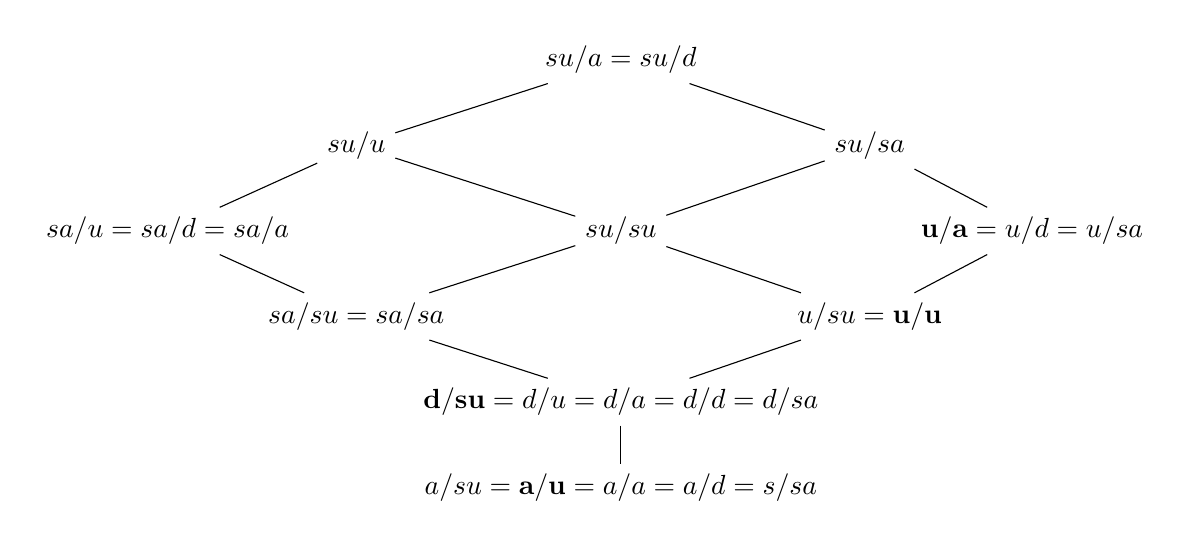
\begin{tikzpicture}
        \matrix[row sep=0.5cm, column sep=-0.5cm] {
            & & \node(13){$su/a = su/d$}; \\
            & \node(22){$su/u$}; & & \node(24){$su/sa$}; \\
            \node(31){$sa/u = sa/d = sa/a$}; & & \node(33){$su/su$}; & & \node(35){$\mathbf{u/a} = u/d = u/sa$}; \\
            & \node(42){$sa/su = sa/sa$}; & & \node(44){$u/su = \mathbf{u/u}$}; \\
            & & \node(53){$\mathbf{d/su} = d/u = d/a = d/d = d/sa$}; \\
            & & \node(63){$a/su = \mathbf{a/u} = a/a = a/d = s/sa$}; \\
        }; 
            
        \graph {
            (13) -- (22);
            (13) -- (24);
            (22) -- (31);
            (22) -- (33);
            (24) -- (33);
            (24) -- (35);
            (31) -- (42);
            (33) -- (42);
            (33) -- (44);
            (35) -- (44);
            (42) -- (53);
            (44) -- (53);
            (53) -- (63);
        };
    \end{tikzpicture}
    \caption{Obermengenbeziehungen der Semantiken}
    \label{fig:supset_semantics}
\end{figure}

\newpage
\section{Probabilistisches Schließen}

\subsection{Definitionen}

\subsubsection{Bedingte Wahrscheinlichkeit}

$$ P(A \, | \, B) = \frac{P(A \cap B)}{P(B)} $$

\begin{align*}
    P(A \cap B) & = P(A \, | \, B) \cdot P(B) \\
                & = P(B \, | \, A) \cdot P(A) \\
                & = P(A) \cdot P(B)             & \text{(wenn $A$ und $B$ unabhängig)}
\end{align*}

\begin{align*}
    P(A \cup B) & = P(A) + P(B) - P(A \cap B) \\
                & = P(A) + P(B) - P(A) \cdot P(B)             & \text{(wenn $A$ und $B$ unabhängig)}
\end{align*}

\subsubsection{Satz von Bayes}

$$ P(A \, | \, B) = \frac{P(B \, | \, A) \cdot P(A)}{P(B)} = \frac{P(A \cap B)}{P(B)}  $$

\begin{align*}
    P(A \, | \, B_1 \cap \dots \cap B_k)    & = \frac{P(B_1 \cap \dots \cap B_k \, | \, A) \cdot P(A)}{P(B_1 \cap \dots \cap B_k)}          & \text{(Verallgemeinerung)} \\
                                            & = \frac{P(A) \cdot \displaystyle \prod_{i=1}^k P(B_i \, | \, A)}{P(B_1 \cap \dots \cap B_k)}  & \text{($B_1, \dots, B_k$ unabhängig)}
\end{align*}

\begin{align*}
                    & P(A_1 \, | \, B_1 \cap \dots \cap B_k) \lessgtr P(A_2 \, | \, B_1 \cap \dots \cap B_k) \\
    \Leftrightarrow & P(A_1) \cdot \displaystyle \prod_{i=1}^k P(B_i \, | \, A_1) \lessgtr P(A_2) \cdot \displaystyle \prod_{i=1}^k P(B_i \, | \, A_2)
\end{align*}

\subsection{Anwendung}

\begin{itemize}
    \item Beispiel Spamfilter
    \item $ P(spam \, | \text{ Congratulations ur awarded}) \lessgtr P(ham \, | \text{ Congratulations ur awarded}) $
    \item Problem, wenn \say{ur} nicht in Trainingsdaten
    \begin{itemize}
        \item $ P(spam \, | \, ur) = \frac{\#(\text{Mails mit \say{ur}})}{\#(\text{Spam-Mails})} = 0$
        \item Gesamtwahrscheinlichkeit wird 0
        \item Laplace-Smoothing: $ P(spam \, | \, ur) = \frac{\#(\text{Mails mit \say{ur}}) + 1}{\#(\text{Spam-Mails}) + |\text{Vokabular}|} $
    \end{itemize}
\end{itemize}

\newpage
\section{Neuronale Netze}

\subsection{Aufbau}

\begin{itemize}
    \item Neuronen
    \begin{itemize}
        \item Inputs
        \item Gewichte
        \item Bias
        \item Output: $y = f_w(x)$ mit Aktivierungsfunktion $f_w$
    \end{itemize}
    
    \item Topologische Anordnung
    \begin{itemize}
        \item Input-Layer
        \item Hidden-Layers
        \item Output-Layer
    \end{itemize}
\end{itemize}

\subsection{Lineare Regression}

\begin{itemize}
    \item $ f_{w_0, w_1}(x) = w_1x + w_0 = y $
    \item Verlustfunktion
    \begin{itemize}
        \item $ \displaystyle Loss(f_w) = \sum_{j = 1}^N(y_j - f_w(x_j))^2 = \sum_{j = 1}^N(y_j - (w_1x_j + w_0))^2 $
        \item $N$: Anzahl Trainingswerte
        \item $x_j$: Argument des $j$-ten Trainingswertes
        \item $y_j$: $j$-ter Trainingswert
    \end{itemize}
    
    \item Verlust minimieren: Geschlossene Lösung
    \begin{itemize}
        \item Minimum von $Loss$ berechnen
        \item $ \displaystyle 0 = \frac{\partial}{\partial w_0} Loss(f_w) = 2 \cdot \sum_{j = 1}^N y_j - (w_1x_j + w_0) $
        \item $ w_0 = \frac{\displaystyle (\sum_{j = 1}^N y_j) - w_1 \sum_{j = 1}^N x_j}{N} $
        \item $ \displaystyle 0 = \frac{\partial}{\partial w_1} Loss(f_w) = 2 \cdot \sum_{j = 1}^N (y_j - (w_1x_j + w_0))x_j $
        \item $ w_1 = \frac{\displaystyle (N \sum_{j = 1}^N x_jy_j) - (\sum_{j = 1}^N x_j) (\sum_{j = 1}^N y_j)}{\displaystyle N (\sum_{j = 1}^N x_j^2) - (\sum_{j = 1}^N x_j)^2} $
        \item meist zu kompliziert $\rightarrow$ \textit{Gradient Descent}
    \end{itemize}
    
    \item Gradient Descent
    \begin{itemize}
        \item Greedy-Ansatz
        \item Gradient
        \begin{itemize}
            \item $ \nabla f(x_1, \dots, x_k) = \begin{pmatrix} \frac{\partial f}{\partial x_1} \\ \vdots \\ \frac{\partial f}{\partial x_k} \end{pmatrix} $
            \item zeigt in Richtung des stärksten Anstieges
            \item Betrag gibt Stärke des Anstiegs an
        \end{itemize}
        \item $ w_0 \leftarrow w_0 - \alpha (\frac{\partial}{\partial w_0} Loss(f_w)) $
        \item $ w_1 \leftarrow w_1 - \alpha (\frac{\partial}{\partial w_1} Loss(f_w)) $
        \item \label{alpha} Schrittgröße $\alpha$
        \begin{itemize}
            \item am Anfang groß wählen ($\sim 0.01$), schrittweise verringern
            \item Schrittweise verringern
            \item zu groß: kein Optimum
            \item zu klein: viele Schritte
        \end{itemize}
    \end{itemize}
\end{itemize}

\subsection{Klassifikation}

\subsubsection{Lineare Klassifikation}

\begin{itemize}
    \item zwei Klassen nach linearer Regression: $C_1, C_2$
    \item $ x_2 = w_1 x_1 + w_0 \Rightarrow w_0 x_0 + w_1 x_1 + w_2 x_2 = 0 $, für $x_0 = 1$ und $w_2 = -1$
    \item $ \begin{pmatrix} w_0 \\ w_1 \\ w_2 \end{pmatrix} \cdot \begin{pmatrix} x_0 \\ x_1 \\ x_2 \end{pmatrix} = \Vec{w} \cdot \Vec{x} = 0 $ Schwellwert
    \item $ \Vec{w} \cdot \Vec{x} < 0 \Rightarrow C_1 $
    \item $ \Vec{w} \cdot \Vec{x} > 0 \Rightarrow C_2 $
    \item Schwellwert als Aktivierungsfunktion $f_w$
    \begin{itemize}
        \item $ f_w(\Vec{x}) = Step(\Vec{w} \cdot \Vec{x}) $
        \item $ Step(x) = \begin{cases} 1 \text{, wenn } x > 0 \\ 0 \text{, wenn } x < 0 \end{cases} $
        \item Problem: $Loss$ nicht differenzierbar
        \item Lösung: $ f_w(x) = Logistic(x) = \frac{1}{1 + e^{-x}}$
        \item $ Logistic'(x) = Logistic(x) \cdot (1 - Logistic(x)) $
    \end{itemize}
    
    \item Gradient Descent
    \item $ f_w(x) = Logistic(x) $
    \begin{itemize}
        \item $ w_i \leftarrow w_i - \alpha \frac{\partial}{\partial w_i} (y - f_w(x))^2 $
        \item $ w_i \leftarrow w_i - \alpha (y - f_w(x)) \cdot f_w(x)(1 - f_w(x)) \cdot (-x_i) $
    \end{itemize}
    
    \item Grenze: Nichtlineare Daten
\end{itemize}

\subsubsection{Nichtlineare Klassifikation}

\begin{itemize}
    \item $L+1$ vernetzte Schichten, $K$ Klassen
    \item Input-Layer: $l=0$
    \item Output-Layer: $l=L$
    \item Neuronen definiert durch
    \begin{itemize}
        \item Layer: $l$
        \item Index: $i, j$
        \item Input für Layer $l$: $h_i^{(l-1)}$
        \item Gewicht für $h_i^{(l-1)}$: $w_{i,j}^{(l)}$
        \item Gesamtinput: $ a_j^{(l)} = \sum w_{i,j}^{(l)} \cdot h_i^{(l-1)} = \Vec{w_j}^{(l)} \cdot \Vec{h}^{(l-1)} $
        \item Aktivierungsfunktion: $h(x)$
        \item Ausgabe: $h_j^{(l)} = h(a_j^{(l)})$
    \end{itemize}
    
    \item Aktivierungsfunktion Softmax
    \begin{itemize}
        \item erhält Wahrscheinlichkeitsverteilung $f$ aus Outputlayer
        \item $Logistic$ in $K$ Dimensionen
        \item $ f_k = \frac{e^{a_k^{(L)}}}{\sum e^{a_j^{(L)}}} \text{ für } k = 1, \dots, K $
        \item $ \displaystyle f_k \in [0, 1] \wedge \sum_{k=1}^K f_k = 1 $
        \item $ f = [f_1, \dots, f_K] $ (Wahrscheinlichkeitsverteilung)
    \end{itemize}
    
    \item Darstellung als Funktion
    \begin{itemize}
        \item $ a_j^{(l)} = \Vec{w_j}^{(l)} \cdot \Vec{h}^{(l-1)} $
        \item Gewichte der Neuronen von Ebene $l$ bilden Matrix $W^{(l)}$
        \item $ a^{(l)} = W^{(l)} \cdot \Vec{h}^{(l-1)} = \begin{pmatrix} w_{1,1} & \dots & w_{K,1} \\ \vdots & \ddots & \vdots \\ w_{K,1} & \dots & w_{K,K} \end{pmatrix}^{(l)} \begin{pmatrix} \Vec{h}_1 \\ \vdots \\ \Vec{h}_K \end{pmatrix}^{(l-1)} $
        \item $ f(\Vec{x}) = f[a^{(L)}(h^{(L-1)}(\dots(h^{(1)}(a^{(1)}(\Vec{x})))))] $
    \end{itemize}
    
    \item Kreuzentropie (siehe \ref{entropy})
    \begin{itemize}
        \item misst Unordnung zwischen $p$ und $q$
        \item $ H(T) = \displaystyle \sum_{i = 1}^K -p_i \cdot \log_2(q_i) $
        \item Bewertung der Ähnlichkeit von $f$ und $y$
        \item $ \displaystyle L(y, f) = - \sum_{i = 1}^K y_i \cdot \log_2(f_i) $
        \item Durchschnittliche Kreuzentropie bei $N$ Beispielen: $ \displaystyle \frac{1}{N} \sum_{j=1}^N L(y_j, f(\Vec{x_j}) $
    \end{itemize}
    
    \item Training
    \begin{itemize}
        \item Trainingsbeispiele $(x, y)$
        \item lerne Gewichte $w_{i,j}^{(l)}$
        \item Gradient von Lossfunvtion zu Hidden Layers $\rightarrow$ Back-propagation
        \item Stochastic Gradient Descent
        \begin{itemize}
            \item Gradienten über alle $N$ Beispiele berechnen $\rightarrow$ zu viel
            \item Gradienten über jeweils ein Beispiel $\rightarrow$ zu wenig
            \item Gradienten über Mini-Batches (z. B. 256)
        \end{itemize}
        
        \item Lernrate $\alpha$ (siehe \ref{alpha})
        \item Overfitting
        \begin{itemize}
            \item zu starke Anpassung auf Trainingsdaten
            \item $accuracy_{training} \gg accuracy_{validation} $
            \item Auswahl der Trainingsdaten randomisieren (90/10 - Trainingsdaten/Validation)
            \item Modellkomplexität (Zahl der Parameter) verringern
        \end{itemize}
    \end{itemize}
\end{itemize}

\subsection{Grenzen}

\begin{itemize}
    \item Netzwerkarchitektur
    \item Lokale Optima, Heuristik
    \item Trainingsdaten
    \item Overfitting
    \item Intransparente Modelle
\end{itemize}

\section{Unsupervised Learning}

\begin{figure}[ht]
    \centering
    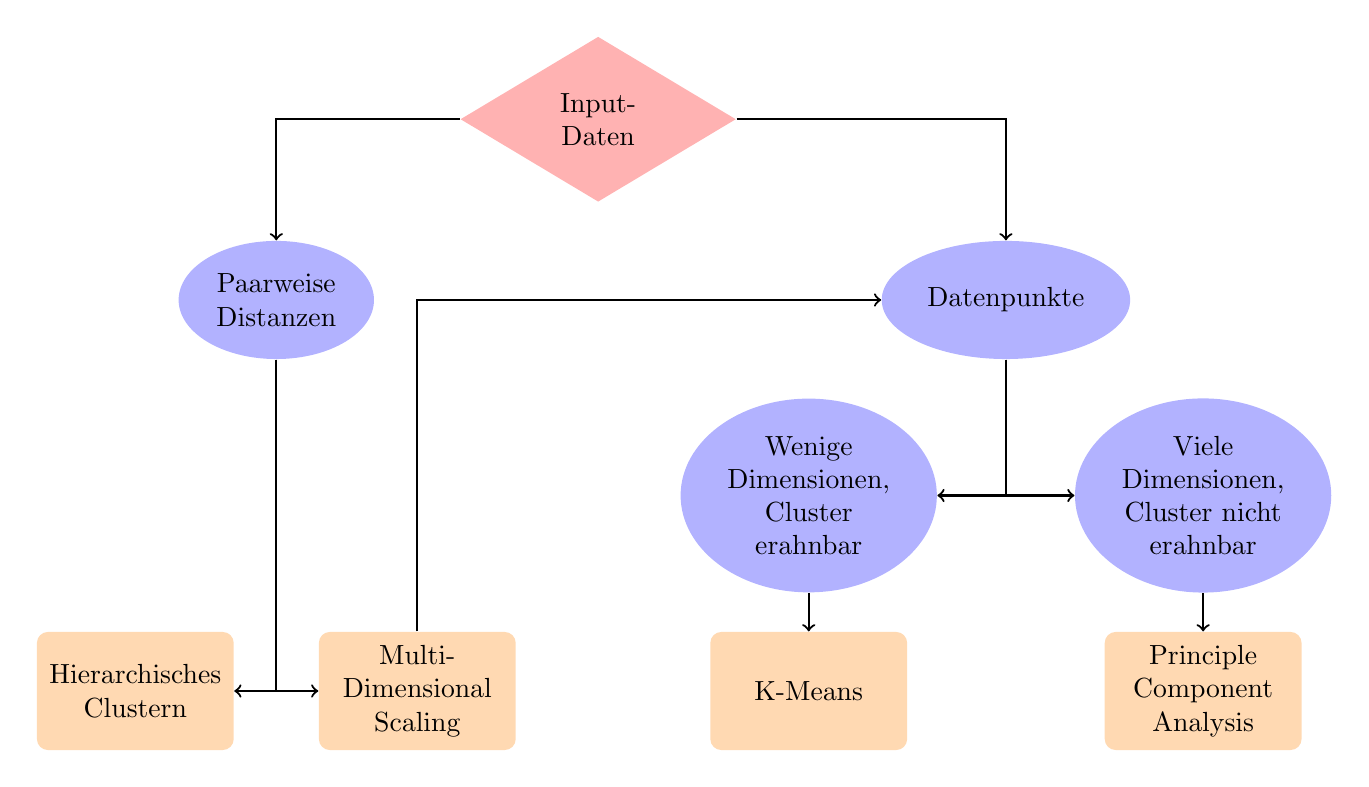
\begin{tikzpicture}
        \matrix[row sep=0.5cm, column sep=-0.7cm]{
            & & & \node[input](14){Input- \\ Daten}; \\
            
            & \node[feature](22){Paarweise \\ Distanzen}; & & & & \node[feature](26){Datenpunkte}; \\
            
            & & & & \node[feature](35){Wenige \\ Dimensionen, \\ Cluster \\ erahnbar}; & & \node[feature](37){Viele \\ Dimensionen, \\ Cluster nicht \\ erahnbar}; \\
            
            \node[method](41){Hierarchisches \\ Clustern}; & & \node[method](43){Multi- \\ Dimensional \\ Scaling}; & & \node[method](45){K-Means}; & & \node[method](47){Principle \\ Component \\ Analysis}; \\
        };
        
        \graph {
            (14) ->[to path={-| (\tikztotarget)}, thick] (22);
            (14) ->[to path={-| (\tikztotarget)}, thick] (26);
            (22) ->[to path={|- (\tikztotarget)}, thick] (41);
            (22) ->[to path={|- (\tikztotarget)}, thick] (43);
            (26) ->[to path={|- (\tikztotarget)}, thick] (35);
            (26) ->[to path={|- (\tikztotarget)}, thick] (37);
            (35) ->[thick] (45);
            (37) ->[thick] (47);
            (43) ->[to path={|- (\tikztotarget)}, thick] (26);
        };
    \end{tikzpicture}
    \caption{Übersicht der Unsupervised-Learning-Methoden}
    \label{fig:unsupervised_learning}
\end{figure}

\begin{table}[ht]
    \centering
    \begin{tabular}{c|c c}
        \toprule
        Methode & Vorteile  & Nachteile \\
        \midrule
        K-Means & 
        \makecell{  
            \tabitem einfach \\
            \tabitem schnell ($O(n)$)
        }   &
        \makecell{
            \tabitem Greedy, kein globales Optimum \\ $\rightarrow$ Bootstrapping \\
            \tabitem Wie viele Cluster $k$? \\
            \tabitem Welches Distanzmaß?
        } \\
        \midrule
        \makecell{Hierarchical \\ Clustering}   &   &
        \makecell{
            \tabitem Komplexität $O(n^3)$ \\
            \tabitem Greedy, kein globales Optimum \\
            \tabitem Welche Linkage-Methode \\
            \tabitem Welches Distanzmaß? \\
        } \\
        \midrule
        \makecell{Principal \\ Component \\ Analysis}   & 
        \makecell{  
            \tabitem einfach \\
            \tabitem Visualisierung \\
            \tabitem Komplexität $O(p^2 \cdot n + p^3)$
        }   &
        \makecell{
            \tabitem Komplexität $O(p^2 \cdot n + p^3)$ \\
            \tabitem $n$ Punkte, $p$ Dimensionen
        } \\
        \midrule
        \makecell{Multi- \\ Dimensional \\ Scaling} &   &
        \makecell{
            \tabitem nicht immer möglich \\ z. B. $ D(A,B) = 1 = D(B,C) $ \\ $ D(A,C) = 5 $
        } \\
        \bottomrule
    \end{tabular}
    \caption{Vergleich der Methoden des Unsupervised Learnings}
    \label{tab:unsupervised_learning}
\end{table}

\begin{itemize}
    \item Supervised
    \begin{itemize}
        \item Beispiele
        \begin{itemize}
            \item Entscheidungsbäume
            \item HMM
            \item Bayes
            \item Neuronale Netze
        \end{itemize}
        
        \item braucht große Mengen an Trainingsdaten
        \item Qualität und Menge reicht oft nicht
    \end{itemize}
    
    \item Unsupervised
    \begin{itemize}
        \item Beispiel siehe \nameref{fig:unsupervised_learning}
        \item braucht keine Trainingsdaten
    \end{itemize}
\end{itemize}

\newpage
\subsection{K-Means}

\begin{itemize}
    \item wähle erste $k$ Elemente als Clusterzentren (Repräsentanten)
    \item weise jedes Element Cluster zu, bei dem sich Varianz am wenigsten erhöht (geringste Distanz zum Clusterzentrum)
    \item Wahl eines neuen Repräsentanten anhand der Elemente im Cluster
    \item wiederholen
\end{itemize}

\subsection{Hierarchical Clustering}

\begin{itemize}
    \item Input: Paarweise Distanzen (Heuristik)
    \item Output: Baum mit Objekten als Knoten
    \item Iteratives mergen der Objekte mit kleinster Distanz
    \item Distanz des neuen Clusters $w = (u, v)$ zu anderen Objekten $x$
    \begin{itemize}
        \item Single/Complete linkage
        \begin{itemize}
            \item \textbf{Single} linkage: $ D(x,w) = \min(D(x,u), D(x,v)) $
            \item \textbf{Complete} linkage: $ D(x,w) = \max(D(x,u), D(x,v)) $
        \end{itemize}
        
        \item \textbf{P}air \textbf{G}roup \textbf{M}ethod using \textbf{A}rithmetic mean (PGMA)
        \begin{itemize}
            \item \textbf{Average} linkage/Weighted PGMA (WPGMA): $ D(x,w) = \frac{D(x,u) \, + \, D(x,v)}{2} $
            \item Unweighted PGMA (\textbf{UPGMA}): $ D(x,w) = \frac{m_u \cdot D(x,u) \, + \, m_v \cdot D(x,v)}{m_u \, + \, m_v} $
            \item $m_u$ ist Anzahl Knoten in $u$
        \end{itemize}
        
        \item Linkage hat Einfluss auf Ergebnis
    \end{itemize}
\end{itemize}

\subsection{Principal Component Analysis}

\begin{itemize}
    \item Mehrere Hauptachsen
    \item Basiswechsel
    \begin{itemize}
        \item rotiert Achsen
        \item $x_1$-Achse entspricht erster Hauptachse, $x_2$-Achse zweiter, usw.
    \end{itemize}
    
    \item Reduktion der Dimensionen $\rightarrow$ Suche der Cluster in kleineren Dimensionen
    \item Voraussetzung: Hoher erklärter Varianzanteil
\end{itemize}

\subsection{Multi-Dimensional Scaling}

\begin{itemize}
    \item Verallgemeinerung der Principal Component Analysis mit messbaren Relationen zwischen Daten
    \item Relationen $\rightarrow$ Koordinaten
    \item Platzierung der ersten Koordinate $A$
    \item Platzierung der zweiten Koordinate $B$ auf Kreis um $A$ mit $ r = D(A,B) $
    \item Sukzessives platzieren der weiteren Knoten auf Schnittpunkten der Kreise um Koordinaten
\end{itemize}

\end{document}
